%\part{Konstruktion}
%\chapter{Programmlogik}
%\section{QueryResolution}

\subsection{QuerySend}

\begin{figure}[htb]
	\centering
  	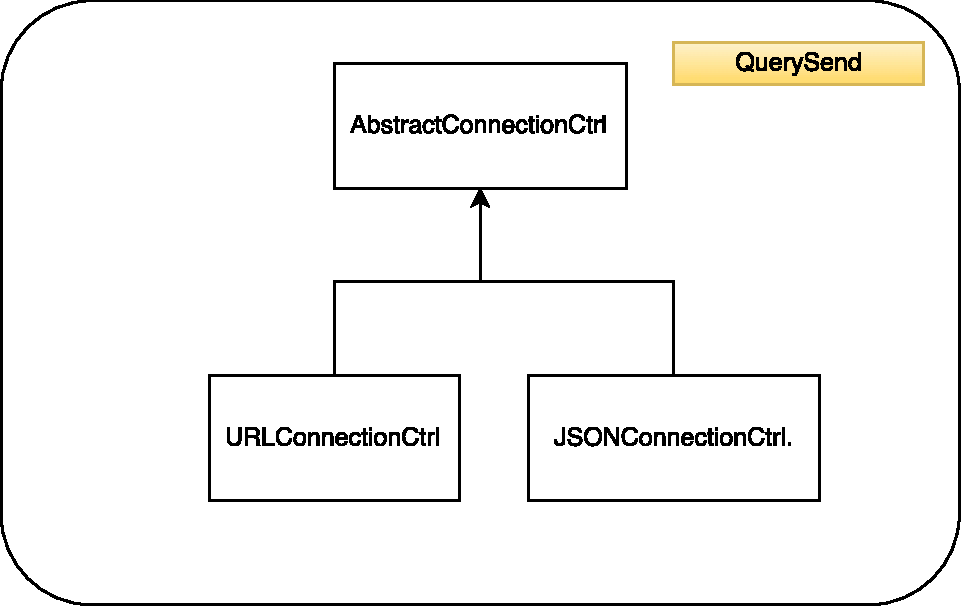
\includegraphics[width=0.8\textwidth]{qr_querysend}
  	\caption{Aufbau des Moduls \lstinline|QuerySend|}
\end{figure}

Im Modul \lstinline|QuerySend| befinden sich die \lstinline|ConnectionController|, die für das Versenden der Anfrage zuständig sind. Sie werden mithilfe von \lstinline|QueryBuild| konfiguriert und erhalten den Parser (\lstinline|ResponseParse|). Vor dem Weiterreichen an den \lstinline|TaskController|, wird durch den Parser noch von NSData zu \lstinline|SearchResult| umgewandelt.